% Life is a compromise anyway

\section{Adapting music for a group of listeners} % (fold)
\label{sec:adapting_music_for_a_group_of_listeners}

% section adapting_music_for_a_group_of_listeners (end)
The first part of the thesis has explained how to use experience data from the Web to perform two specific tasks: estimate musical association between songs %from a set of playlists 
(Chap.~\ref{cha:smoothness}) and estimate individual music preferences % from listening habits 
(Chap.~\ref{cha:preferences}).

Musical associations (which songs or artists sound well together in sequence) and individual preferences (what the public would like to hear) serve as the basis for the technique described in this chapter, which represents the main contribution of this dissertation.
This technique helps identify, in a large repository of music, a subset of songs adapt for a group of listeners.

While disc jockeys (DJs) can use their senses to perceive the taste of the audience (watching their reaction, listening to their requests) and know from experience which songs mix well one after the other, here the methods introduced in the first part of the thesis % to identify musically associated songs and individual music preferences 
are used to deliver group-customised music sequences (see Fig.~\ref{fig:schema}).
%
\begin{figure}[bthp]
\centering \setlength{\abovecaptionskip}{3pt}
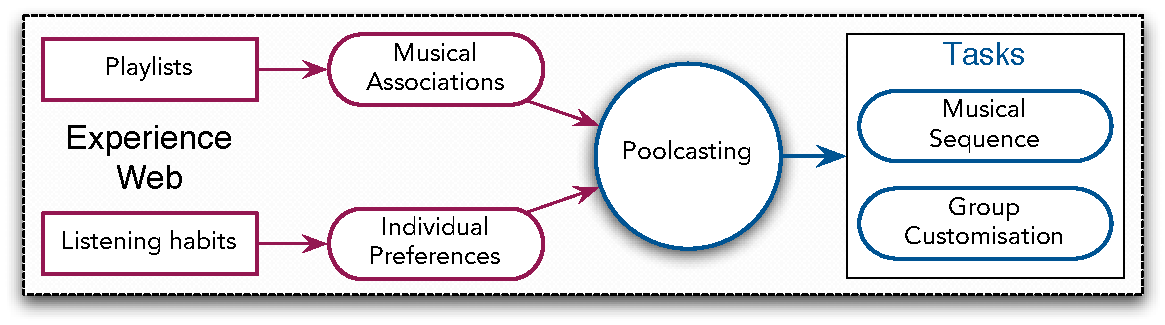
\epsfig{file=img/fig4_1, width=\textwidth}
\caption{Collecting music experiences from the Web to deliver sequences of songs customised for groups of listeners.}
\label{fig:schema}
\end{figure}

\subsection{Problem Definition} % (fold)
\label{sub:problem_definition2}

There are several situations where groups gather to listen to music, such as home parties, discos and, in a virtual sense, radio stations.
In these contexts, someone is entitled to decide \emph{which} songs to play; this can either be a professional DJ or someone from the audience.

%The goal of this chapter is to present a family of techniques called poolcasting that `behave like a good DJ', selecting from a possibly large repository of music a subset of songs that best satisfy the current audience.

In discos and AM/FM radios, expert DJs are appointed to select the best music for the audience. 
In home-parties, bars and online radios, this task is instead typically left in the hands of an automated system, for instance a portable music device (Apple iPod) with the `shuffle' option turned on.

The problem with \textbf{automated music selection} is that the preferences and reactions of the audience are not considered, so the result can be unsatisfactory for the actual listeners. Moreover, an automated selection does not ensure that each played song `sounds well' after the previous one.

The problem addressed in this chapter is whether an intelligent technique can `act as a good DJ', autonomously adapting the music to the listening audience.
Precisely, the goal is to automatically select and deliver a musical sequence that matches four requirements:
 
{\setlength{\leftmargini}{42pt} 
\begin{enumerate}
\renewcommand{\theenumi}{Goal \arabic{enumi}}
%\item\label{p:variety} \textbf{Variety}: the same song or songs by the same artist should be not played multiple times at close distances;
%\item\label{p:smoothness} \textbf{Smoothness}: each song should form a smooth musical transition with the previously played song;
%\item\label{p:customisation} \textbf{Customisation}: each song should match the music preferences of the current listeners; and
%\item\label{p:fairness} \textbf{Fairness}: the whole musical sequence should ensure, in the long run, an equal degree of satisfaction to all the listeners.
\item\label{p:variety} \textbf{Variety}: no song or artist should be repeated within a short period of time;
\item\label{p:smoothness} \textbf{Smoothness}: songs should follow a sequence perceived as musically smooth;
\item\label{p:customisation} \textbf{Customisation}: songs should match the musical interests of the current audience; and
\item\label{p:fairness} \textbf{Fairness}: in the long run, every listener should have a similar degree of satisfaction with respect to the music played.
\end{enumerate}
}
The first two properties are meant to build a good sequence of songs, avoiding repetitions (\ref{p:variety}) and ensuring a certain musical continuity (\ref{p:smoothness}).
The last two properties are meant to customise the music for the group: selecting songs according to the musical taste of the audience (\ref{p:customisation}) and embracing the preferences of every listener in the long run (\ref{p:fairness}).

% subsection problem_definition2 (end)

\subsection{The poolcasting approach} % (fold)
\label{sub:what_is_poolcasting}

This chapter presents poolcasting, an intelligent technique that addresses the music selection problem described above.
Poolcasting generates musical sequences in real time, selecting at each moment which songs to play next based on the current audience and on the set of available songs.



The way in which the four goals of of variety, smoothness, customisation and fairness are addressed is by means of a Case-Based Reasoning (CBR) process that identifies which song to play at each moment.

CBR systems, given a new problem to solve, first \emph{retrieve} similar past problems, then \emph{reuse} their solutions to generate a good solution for the new problem, finally \emph{revise} the proposed solution.
Similarly poolcasting, to select at a given moment which song to play on a channel:
\begin{enumerate}
 \item \emph{(Retrieve Process)} first retrieves a subset of available songs (the retrieved set) that have not been played recently (\ref{p:variety}) and form a smooth musical transition with the last song played (\ref{p:smoothness});
 \item \emph{(Reuse Process)} then ranks the retrieved set according to the preferences of the current audience (\ref{p:customisation}) giving more importance to those listeners less satisfied with the music recently played (\ref{p:fairness}); and  
% \item \emph{(Reuse Process)} then ranks the retrieved set according to the preferences of the current audience (\ref{p:customisation}), identifies in this ranking a song that will keep all the listeners similarly satisfied (\ref{p:fairness}) and selects that song to play next;
 \item \emph{(Revise Process)} finally considers the listeners' feedback to adjust individual preferences % and musical associations 
over time.
\end{enumerate}

In order to know which songs form smooth musical transitions, poolcasting integrates the co-occurrence analysis process introduced in Chap.~\ref{cha:smoothness}. In order to know the preferences of the current audience, poolcasting integrates the implicit user modelling approach described in Chap.~\ref{cha:preferences}. 

% As a result, poolcasting can create musical sequences customised for the listening audience, that achieve the four required goals of variety, smoothness, customisation and fairness.

The rest of the chapter is organised as follows.
Section~\ref{sec:previous_works4} reviews previous work related to Case-Based Reasoning, group-adaptive systems and social choice problems.
%
The CBR process that combines experience knowledge from the Web to customise music for an audience is presented in Sect.~\ref{sec:the_case_based_reasoning_selection_process}.
%
Section~\ref{sec:social-choice-problem} explains how poolcasting can fairly satisfy the entire audience when listeners have different musical tastes.

%Section~\ref{sec:what_i_have_done} describes a Web application providing an online radio service where the poolcasting techniques are employed. This Web radio offers interactive features and social component that stand ahead of existing online radio services.


% The approach of poolcasting to possibly satisfy the \emph{whole} audience is described in Sect.~\ref{sec:social-choice-problem} and consists in achieving fairness in the long run among different listeners.

% subsection from_the_technique_to_the_application (end)




%For instance, if five persons are listening to Rock channel and they all love Electronic Rock and detest Heavy Metal, then poolcasting will take these interests into consideration to decide which Rock track to play next.


% subsection what_is_poolcasting (end)




\section{Previous work} % (fold)
\label{sec:previous_works4}

The approach described in this chapter reinterprets an artificial intelligence technique called Case-Based Reasoning (CBR) which is reviewed hereafter. Previous works on user-adaptive systems are then reported, with special focus on systems that adapt content to groups and have addressed the problem of customising music for an audience.
%Since the architecture of poolcasting is similar to online radios, Internet radios are also reviewed.

\subsection{Case-Based Reasoning} % (fold)
\label{sub:case_based_reasoning_approaches}

% subsection case_based_reasoning_approaches (end)

Case-Based Reasoning \cite{Kolodner93,Aamodt94,LopezDeMantaras05} is the process of problem solving based on the exploitation of past experiences, called cases, to propose solutions for present problems. 
Inspired by cognitive sciences, Case-Based Reasoning is based on the assumption that similar problems have similar solutions. 

In CBR systems, knowledge is typically represented as a library of cases, also called case base.
Each case holds knowledge related to a specific situation and is usually made of a (problem $\rightarrow$ solution) pair: the problem describes a task solved in the past and the solution explains how the task was carried out. 
New tasks can be solved adapting past solutions, following a cycle that comprises four processes: 
\begin{enumerate}
  \item Retrieve: extract from the case base a subset of cases that present problems similar to the current one;
  \item Reuse: adapt the solutions of the retrieved cases to the context of the current problem in order to generate a new solution;
  \item Revise: evaluate and improve the outcome of applying the proposed solution to the current problem; and
  \item Retain: store the newly generated (problem $\rightarrow$ solution) pair in the case base as a new case.
\end{enumerate}

CBR has been applied in distinct domains where similar problems have similar solutions. % and can hardly be FACED with other types of knowledge or rules.
In jurisprudence, for instance, the outcome of a lawsuit strongly depends on past court decisions; a valuable CBR system has been developed with a large case base of historical sentences that are retrieved and reused to help lawyers predict the verdict of new lawsuits \cite{Weber97}.

Another area where CBR has proven helpful is medical diagnosis; CBR systems have been used to diagnose cancer \cite{Diaz06} and Alzheimer's disease \cite{Marling01} comparing data and symptoms of each new patient (current problem) with data and symptoms of previous patients (past problems) who received specific cures (past solutions).

The minimal components of a Case-Based Reasoning system are the retrieve and the reuse steps, which generate a solution for a given problem. 
The main challenge in these steps is how to measure similarity between cases. %
The similarity measure depends on the problem description, ranging from a simple metric that corresponds to the distance between two features to more complex measures that depend on the application domain.

CBR techniques have also been employed in user-adaptive systems, delivering customised content to different targets based on previous interactions with the system.

%The Revise and Retain processes are related to the learning process of the system and are not present in every CBR system.

% \subsection{CBR recommender systems} % (fold)
% \label{sub:examples_of_cbr_rs}
% 
% % subsection examples_of_cbr_rs (end)
% 
% 


% section previous_works4 (end)

\subsection{User-adaptive techniques} % (fold)
\label{sub:user_adaptive_systems}
%(rec/delivery, ..)
%What I want to do is a user-adaptive system. There are different kinds. And what I do does DELIVERY, (while the previous chapter is rec.) of nature MUSIC, outputting a SEQUENCE, targetted to INDIVIDUALS, using a KNOWLEDGE-BASED technique [!! Note, change 2.1.5 into CF, content-based or KB, where is CBR], and CONTINUOUS.


User-adaptive techniques analyse the behaviour of their users, infer a model of their preferences and goals, and deliver content tailored upon their interests. 
%
These techniques have been applied to % domains others than music, for example to 
offer the right level of medical information according to the needs of individual patients \cite{Hirst97}, to adjust educational presentations according to the expertise of the learners \cite{Hohl96}, to give the right support to software users according to their usage \cite{Horvitz98}, to tune the toughness of tracks in a car racing game according to the player's skill \cite{Togelius06}.

User-adaptive systems have also appeared in literature labelled as adaptive interfaces, personalisation systems, adaptive hypermedia systems, user modelling systems, software agents or intelligent agents, and grow on the idea that it is worthwhile to learn something about each individual and adapt the response in some nontrivial way \cite{Brusilovsky01,Montaner03}. 
%Different taxonomies of user-adaptive systems have been proposed \cite{Dieterich93, Brusilovsky96}.
%Adaptation is mostly useful when a system is expected to be used by people with different goals and knowledge. % \cite{Brusilovsky96}
%
% Goal? Task simplification, to sell more, etc

%User-adaptive systems can be classified according to different dimensions.
%The taxonomy proposed in \cite{Dieterich93} classifies user adaptive interfaces according to the stages, agents, constituents, information considered, goals, strategies, levels, and methods of adaptation.
%A shorter taxonomy is presented in \cite{Brusilovsky96}, where four basic dimensions are identified to classify adaptive hypermedia techniques: adaptation tasks, application area, technologies of adaptation and user modelling approach.
% Hereafter, user-adaptive systems are reviewed according to a novel taxonomy that combines elements of the previous two, and categorises systems according to six dimensions: adaptation task, application domain, outcome type, adaptation technique, user modelling approach and learning component.

\subsubsection{Task: recommendation or delivery} % (fold)
\label{ssub:to_recommend_or_to_deliver}

User-adaptive systems can be distinguished according to their task being \emph{recommendation} or \emph{delivery}. A recommender system \emph{suggests} some content of interest,
% (e.g., stating that you should read a specific book, listen to a particular album), 
while a delivery system \emph{delivers} the actual customised content. % (e.g., playing a specific song, broadcasting a particular video). 
\begin{figure}[bthp]
\centering \setlength{\abovecaptionskip}{3pt}
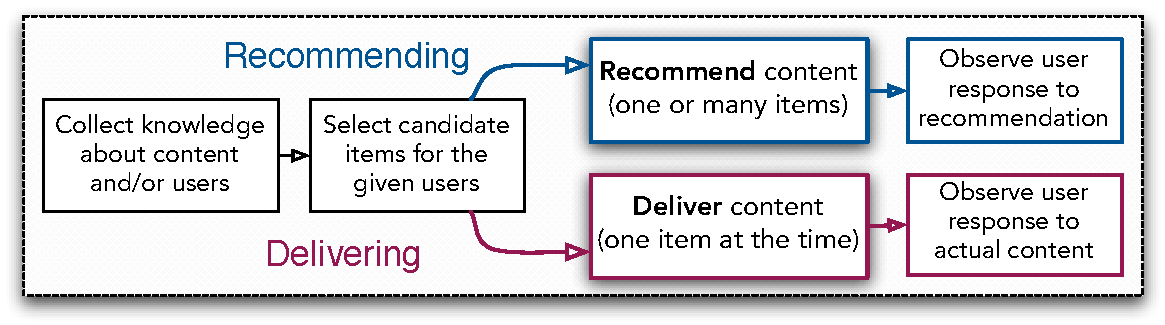
\epsfig{file=img/fig4_2, width=\textwidth}
\caption{Recommender and delivery systems compared.}
\label{fig:recommend_deliver}
\end{figure}

Recommender systems have gained wide attention in relation to the expansion of the World Wide Web, where they have proven helpful for people looking for new movies to watch \cite{Hill95}, songs to listen to \cite{Shardanand94}, news to read \cite{Resnick94}, pages to visit \cite{Lieberman95}, restaurants to check \cite{McCarthy02}, people to know \cite{Terveen05}. %, and in other Web-related applications \cite{Brusilovsky07}.

Delivery is appropriate when items are small, cheap, easily available and storable (e.g., digital audio, digital video, news stories) while items that are large, expensive or not easily available are only recommended (e.g., travel destinations, restaurants, social partners).
Recommender systems can also work on multiple domains at the same time, like InterestMap \cite{Liu05} which simultaneously recommends books, songs, foods, films, television shows and sports based on cross-domain user taste profiles.

Recommender systems often offer unrequested recommendations; for example Amazon constantly presents lists of `recommended books' that customers can completely (and often do) ignore.
By contrast, delivery systems need be prompted by the users for customised content. % to experience. % `on the spot'. For instance, the Web-based music community Last.fm offers personalised radio channels to those users who explicitly ask for a listening experience adapted to their taste.

Since recommender systems do not provide the actual content, an immense collection of items can be recommended without the need for any physical storage. 
For example, MovieLens \cite{Cosley03} recommends movies from a catalogue of 5,600 titles; since movies are recommended\,---\,not delivered\,---\,the system only has to store and transmit the names of the movies, not the real movies.
On the contrary, delivery systems usually require storage and transportation capacity which can limit the range of offer.
%For example, Last.fm personalised radio requires physical space to store the songs, network bandwidth to stream, and a batch process to continuously include newly published songs to the catalogue.

% subsubsection to_recommend_or_to_deliver (end)

\subsubsection{Output: items, sets or sequences} % (fold)
\label{ssub:adaptation_size_and_output}

The outcome of an adaptive system can either be \emph{one} item, a \emph{set} of items, or an ordered \emph{sequence} of items.
%
One item is typical returned when items are expensive (e.g., travels, houses), and the audience can only afford to experience one. 
An example is CATS \cite{McCarthy06b}, which recommends \emph{one} skiing travel destination for a group of friends.

A set of items is commonly returned when items require some time to be experienced (e.g., movies, books). %, and the order in which they are experienced is not paramount. 
For example, MovieLens recommends a \emph{set} of movies to watch and Amazon recommends a \emph{set} of books to read, leaving the users to choose which items to buy and in which order. 
%\cite{Dieterich93} named these systems \emph{user-controlled} adaptive systems.

Finally, a sequence of items is returned when items require a short time to be experienced (e.g., songs, news stories), and the order in which they are experienced is significant. 
For example, Pandora delivers user-adapted Web radio channels with a specific `musical continuity', in the sense that every song is acoustically correlated with the previous song played on the same channel.
% ssubsection adaptation_size_and_output (end)


% [[POTREI TOGLIERE DEL TUTTO QUESTO]]
% \subsubsection{Timing: a priori or continuous} % (fold)
% \label{ssub:timing_continuous_or_discrete}
% 
% User-adaptive systems can either update or not the knowledge content used for the adaptation process. 
% Content-based filtering technique typically estimate all the item-to-item similarity measures beforehand, and do not change them even if users do not appreciate the adaptation proposed. For example, NewsWeeder \cite{Lang95} recommends news stories based on a similarity measure between news item and news item calculated \emph{a priori} using a TF-IDF (Term Frequency - Inverse Document Frequency) approach. Once this measure has been defined, the recommendations are calculated \emph{off-line}, and are not influenced by the user feedback.
% 
% On the contrary, other adaptive systems take into account the response of the audience to improve the customisation on the run. This is mostly true in delivery systems, where immediate user feedback can be obtained to learn whether the adaptation process matched the preference of the public. For example, Pandora.com broadcasts personalised Web radio stations; the selection of the musical sequence is initially focused on maintaining a musical continuity from song to song but, as long as a user starts rating or skipping the proposed songs, the system integrates the user preference in the adaptation algorithm and improves in real time the process producing an even better customised musical stream.

% subsubsection timing_continuous_or_discrete (end)


% subsection user_adaptive_systems (end)


\subsection{Recommender techniques} % (fold)
\label{sub:adaptation_techniques_item_based_and_user_based}

Adaptive systems provide users with content of interest from a potentially overwhelming set of choices.  
Adaptation processes are characterised by different kinds of knowledge representation. % \cite{Brusilovsky96}
A common family of techniques for adaptation is \emph{collaborative filtering}, which consists in presenting a user with content liked by people with a similar profile.
Another family of techniques is called \emph{content-based filtering} and takes place by presenting a user with content similar to items previously liked by the same user.
A third family of techniques, called \emph{knowledge-based}, uses domain knowledge about items' association.

\subsubsection{Collaborative filtering} % (fold)
\label{ssub:collaborative_filtering}

Collaborative filtering techniques select items based on the correlation between people with similar preferences. 
The name ``collaborative filtering'' was proposed by the developers of Tapestry \cite{Goldberg92} and has been used ever since.
The way in which similarity between users is computed depends on the application domain: Amazon interprets similar users as customers who bought the same books in the past, MovieLens as users who rated the some movies likewise.
Once a similarity measure has been defined, the technique works by selecting for each user a set of items liked by people similar to that user.
An interesting comparison of several music-related collaborative filtering systems (Last.fm, Pandora, GhanniMusic, Jango, MeeMix) is presented by \citet{Fox07}.
% COULD REMOVE THIS IMAGE
%\begin{figure}[hbtp]
%\centering \setlength{\abovecaptionskip}{3pt}
%\epsfig{file=img/collaborative_filtering, width=\textwidth}
%\caption{Collaborative filtering.}
%\label{fig:collaborative-filtering}
%\end{figure}


Collaborative filtering is content-agnostic in the sense that the technique is suitable independently of the application domain (e.g., books, music, video).
\citet{Herlocker04} discussed different problems of this approach related to the fact that items cannot be recommended unless users have expressed a preference for them. 
\emph{Cold start} refers to the situation where new items appear and the technique cannot immediately recommend them, since no user rating is available to work on. 
Similarly, when new users join in, the technique needs to learn their preferences before any recommendation can be given. 
\emph{Scarcity} refers to situations where the number of available items is so much larger than the number of users that the coverage of ratings is very sparse and only a few objects are recommendable. 
Another typical problem is for users with \emph{boundary taste} to be provided with poor recommendations since their profiles do not match many other user profiles. 
\emph{Lack of diversity} refers to situations where a collaborative filtering technique suggests a set of items that are intrinsically similar (e.g., five books by the same author, five travels with the same destination) reducing the range of recommendations to a very specific target. 

% subsubsection collaborative_filtering (end)

\subsubsection{Content-based filtering} % (fold)
\label{ssub:content_based_filtering}

Content-based filtering techniques analyse the intrinsic content of every available item and recommend items which are similar to items the user likes. 
The way in which similarity between items is computed depends on the nature of items.
InformationFinder assessed similarity between Web documents comparing the presence of significant phrases \cite{Krulwich96}, while NewsWeeder measured similarity between news stories comparing the frequency of the occurring words \cite{Lang95}.

%Once a similarity measure has been defined, the technique works by selecting for each user a set of items similar to content the user likes.
%% COULD REMOVE THIS IMAGE
%\begin{figure}[hbtp]
%\centering \setlength{\abovecaptionskip}{3pt}
%\epsfig{file=img/content_filtering, width=\textwidth}
%\caption{Content-based filtering.}
%\label{fig:content-based-filtering}
%\end{figure}

Examples of music content-based recommender systems are Mufin, %\footnote{\url{http://mufin.com}}, 
which calculates the similarity between songs comparing properties like tempo, instruments, sound density or harmony \cite{Mufin08}, The Echo Nest, %\footnote{\url{http://the.echonest.com/}}, 
which combines text analysis, audio analysis and user activity \cite{EchoNest09}, and Tangerine, %\footnote{\url{http://www.potionfactory.com/tangerine/}}, 
which works by analysing the BPM and the beat intensity of songs \cite{Tangerine09}.

Content-based filtering is tightly related to the nature of the items to adapt and can obtain good results only in domains where content analysis, parsing and classification have advanced (e.g., text, music), while for complex domains where automatic analysis and categorisation is not yet feasible (e.g., video, interaction data), this is not a suitable approach, since similarities from item to item cannot be drawn as easily.

% subsubsection content_based_filtering (end)

\subsubsection{Knowledge-based techniques} % (fold)
\label{ssub:hybrid_filtering}

Knowledge-based techniques reason about domain knowledge to find items that best match the user needs.
These techniques do not rely on a base of user ratings and are independent of individual tastes.
Instead they have knowledge about how a particular item meets a particular user need, and can therefore reason about the relationship between a need and a possible recommendation \cite{Burke00}.

% From Chun "'THE IMPLEMENTATION OF KNOWLEDGE-BASED RECOMMENDER SYSTEM FOR ELECTRONIC COMMERCE USING JAVA EXPERT SYSTEM LIBRARY"

As \citet{Chun01} pointed out, knowledge-based techniques are appropriate for products like cars, houses, computers, that a person would buy because of knowledge about how an item matches personal requirements rather than because other persons bought that same item.

A music-related knowledge-based system is the Music Genome Projects \cite{Pandora06}.
As a group of trained music analysts listen every day to hundreds of songs and describe their musical qualities ``using up to 400 distinct musical characteristics'', a large knowledge base is built up of relationships between popular themes that serves as the basis for the recommendations provided through Pandora Web radio. % [CITE?].

A sub-category of knowledge-based techniques is composed by % Knowledge-Intensive 
systems that apply Case-Based Reasoning to the task of recommendation.
In these systems, solutions to past problems constitute the knowledge required to provide recommendations for new users.
\citet{Smyth07} summarised advantages of case-based recommender systems, which can converse with the users to better focus on their requirements, evaluate critiques, enhance the diversity of the outcome and explain the reason behind the provided recommendations.
Examples of Case-Based Reasoning recommender systems are Entree \cite{Burke97}, the Wasabi Personal Shopper \cite{Burke99}, Expertclerk \cite{Shimazu01}, WEBSELL \cite{Cunningham01}, Smart Radio \cite{Hayes01b} and the CATS group recommender \cite{McCarthy06b}.


% from burke00


\subsection{Group-adaptive systems} % (fold)
\label{sub:group_adaptive_systems}

Adaptive systems can either be targeted to individuals or to groups.
Extending adaptation processes to groups is a challenging problem, since each member has particular characteristics that should be accounted for. 
\citet{Messick83} pointed out how a group-adaptive system faces the ``social dilemma''  of looking for a compromise between individual and collective interests. 
The system has to find the behaviour that is adequate for the group while taking into account individual preferences of each member.

Group-adaptive systems have appeared in domains other than music, for instance \citet{McCarthy02} described a system that advices a group of friends with a restaurant to attend, \citet{OConnor01} a movie to watch, \citet{McCarthy06b} a tourist attraction to visit. % In all these situations, recommender systems need decide among different options, whereas the members of the group can have heterogeneous preferences towards these options.

The way in which adaptation for the group takes place depends on the characteristic of the group.
\citet{Hill95} distinguished between \emph{co-located} and \emph{displaced} groups.
In the last case, the term ``virtual community'' is more appropriate: people can influence each other as though they interacted but they do not interact, and the system has to maintain displaced members aware of the actions and decisions taken by the group.

\citet{Haseman02} distinguished between \emph{changing} and \emph{stable} groups, meaning that members are allowed or not to join and leave the group. If the composition of a group changes with time, a group-adaptive system might need to inform new members about how previous decisions were made.

\citet{Saklofske89} and \citet{Raghunathan08} remarked how people in a group feel a sense of affiliation with the others and this can positively influence enjoyment from sharing a hedonic activity.
While \emph{intentional} groups take place when people explicitly long for a social experience to share with other people, % for instance when they decide to watch TV with their family, or go dancing with their friends. 
\emph{accidental} groups are made of people who gather with no explicit reason.
\citet{McCarthy98} presented an example of how hard it is to satisfy an accidental group.

%People who do not like Rap music might as well listen to some Rap radio if this makes a friend happy, but they would not do the same for the sake of some complete stranger. 

People in accidental groups are \emph{competitive}, trying to push their individual goals in front of everyone else's, as in political elections. 
In intentional groups, people are instead more \emph{collaborative}, trying to reach a certain degree of group satisfaction.
Intentional groups are generally small groups for which sociologists have found that members may give up part of their individual goals to reach for some group effects, such as conformity, cohesiveness and ``consensuality'' \cite{Hogg96}.

\citet{Chae98} used the term ``narrowcasting'' to describe the situation where media content is delivered to a small group.
In a narrowcasting scenario, people are able to select from a long list of customised channels rather than passively experience a generic broadcast content.
Narrowcasting enables the audience to precisely match the experience with their own views, although \citet{Chaffee01} pointed out how this confines people to live in a ``cocoon of self-reinforcing media''. 

% subsection group_adaptive_systems (end)


\subsection{Preference aggregation} % (fold)
\label{sub:preference_aggregation}

The main challenge for a group-adaptive system is how to combine preferences of multiple persons when they differ.
There are distinct models to aggregate multiple individual preferences in order to assess the ``suitability'' \cite{Jameson07b} of a particular item for a group as a whole. 

Preference aggregation is a multi-person decision making problem that has been broadly covered by social choice theorists \cite{Arrow70}, social psychologists, economists and information scientists \cite{Tindale03,List02}.

% Enric says: we view this as a social choice problem (?)

 %, and has been shown that no judgement aggregation function exists generating ``complete, consistent and deductively closed collective sets of judgements which satisfies universal domain, anonymity and systematicity'' \cite{List02}.

% \begin{figure}[hbtp]
% \centering \setlength{\abovecaptionskip}{3pt}
% \epsfig{file=img/pref_aggr_1, width=\textwidth}
% \caption{Aggregating preferences to select one candidate.}
% \label{fig:preference-aggregation}
% \end{figure}

% Social choice theory aims at finding rules for amalgamating different preferences to ensure certain `desirable properties' \cite{Grabisch98} of the resulting group choice. 

Different approaches proposed to aggregate group preferences include:
introducing social functions that employ some pre-defined aggregation strategy \cite{Masthoff04};
asking users to provide information to determine how the combination can be accomplished \cite{Jameson04};
asking domain experts to guide the combination process \cite{Ardissono03};
promoting social interaction with an interface that allows people to watch, critique, suggest, and discuss recommended items \cite{McCarthy06b}; 
deputing to agent negotiation, with automated agents acting on behalf of humans to generate and form group recommendations \cite{Bekkerman06};
modelling information markets through which group members bet on their judgement about future events \cite{Sunstein05};
developing genetic algorithms \cite{Holland75} to identify the item that best combines individual and group ratings \cite{Chen08}.


%% subsection preference_aggregation (end)

%\subsection{Criteria of fairness} % (fold)
%\label{sub:fairness_of_aggregation_models}

The election of an aggregation function to merge individual preferences is conditioned by the required level of fairness.  
Depending on the application, various rationality principles may apply to select alternatives.

When aggregating multiple individual preferences into a unique group choice, a number of goals are desirable but not always compatible among them, such as matching the preference of the majority, preventing people from leaving the group, maximising average satisfaction, ensuring some degree of fairness, treating group members differently when appropriate, discouraging manipulation of the recommendation mechanism, ensuring comprehensibility and ``acceptability'' \cite{Jameson07b} and minimising misery.
Misery refers to the situation where at least one member of the group is strongly unsatisfied by the aggregation made.

\citet{Chevaleyre07} illustrated different approaches to achieve a degree of fairness in the group, such as \emph{egalitarianism} and \emph{utilitarianism}. 
An egalitarian allocation is driven by the individual utility of the \emph{poorest} agent in the system; aiming at maximising this value is an example for a basic fairness requirement.
An utilitarian allocation is driven by the \emph{sum} of the individual utilities; asking for maximal utilitarian social welfare is a very strong efficiency requirement. 

The weakest possible requirement for preference aggregation is \emph{Pareto efficiency} \cite{Grabisch98}: if at least one individual prefers an item $X$ to an item $Y$ and no one likes $Y$ better than $X$, then the aggregated preference of the group should be higher for $X$ than for $Y$.

Criteria of fairness change when the group-adaptive system does not select \emph{one} item, but rather delivers a whole \emph{sequence} of items, customised for the group.
Behavioural decision theory \cite{Novemsky05} suggests that the mere fact that an outcome is embedded in a sequence might create a frame of reference that can influence subsequent preferences.
In these cases, the history of past aggregations should be taken into account to promote fairness. 
% This is done by Flycasting.

% \begin{figure}[hbtp]
% \centering \setlength{\abovecaptionskip}{3pt}
% \epsfig{file=img/pref_aggr_2, width=\textwidth}
% \caption{Aggregating preferences to select a sequence of candidates.}
% \label{fig:preference-aggregation-sequence}
% \end{figure}

% subsection fairness_of_aggregation_models (end)


%\section{Customising a radio channel for its audience} % (fold)
%\label{sec:what_i_want_to_do}

%\subsection{Problem definition} % (fold)
%\label{sub:problem_definition}

% subsection problem_definition (end)

%The goal of poolcasting is to broadcast on each channel a sequence of songs that is satisfactory for the group of listeners.
%Poolcasting generates this sequence by adding in real time one song after the other. 

%This selection process is driven by four requirements that every played song should match:


% \subsection{Fairness} % (fold)
% \label{sub:aggregating_multiple_preferences2}
% 
% [This subsection should be revised]
% 


\section{The Case-Based Reasoning selection process} % (fold)
\label{sec:the_case_based_reasoning_selection_process}

Poolcasting is a technique to adapt musical content for a group, and is focused around the idea of \textbf{channel}.
A channel represents the virtual space where a group of people gather to listen to music together: a radio channel, a party location, a discotheque.

The persons listening to a particular channel are called the \textbf{audience} of the channel and are indicated with $\mathcal{U}$. 
People are free to join and abandon a channel at different moments: the audience of a channel changes with time. 

The notation $\mathcal{U}_T \subseteq \mathcal{U}$ refers to the set of persons in the channel at a given time $T \in \mathbb{N}^+$ where time is measured counting the songs played so far on the channel: $\mathcal{U}_1$ denotes the audience of the channel while the first song is playing, $\mathcal{U}_2$ while the second song is playing, and so on.

The set of songs available to be played form the \textbf{content} of the channel and are indicated with $\mathcal{C}$.
Similarly to the audience, content can change with time; for instance newcomers can bring more CDs to a party or a radio can buy new records.
The songs available at a particular time  $T \in \mathbb{N}^+$ are indicated with $\mathcal{C}_T \subseteq \mathcal{C}$.

The problem addressed by poolcasting is to play a sequence of songs that matches the four goals of variety, smoothness, customisation and fairness introduced in Sect.~\ref{sec:adapting_music_for_a_group_of_listeners}.
Since both the audience and the content change over time, the musical sequence cannot be entirely scheduled at time $T = 0$ but has to built in real time considering at each moment the available songs and current participants.

%The notation $H_T$ is used to indicate which song is played at time $T$.
Poolcasting follows an \textbf{iterated} decision approach: 
while the first song is playing on the channel, poolcasting decides which will be the second song to play; as soon as the first song ends, the second song starts playing on the channel and poolcasting decides which song will play next, and so on.
%
The way in which poolcasting determines which song to play at any given moment $T$ is by means of a CBR process that is represented in 
Fig.~\ref{fig:iterative_cbr} and whose components (case bases, retrieve, reuse, revise process) are explained hereafter.
%
\begin{figure}[bthp]
\centering \setlength{\abovecaptionskip}{3pt}
%\epsfig{file=img/iterative_cbr, width=\textwidth}
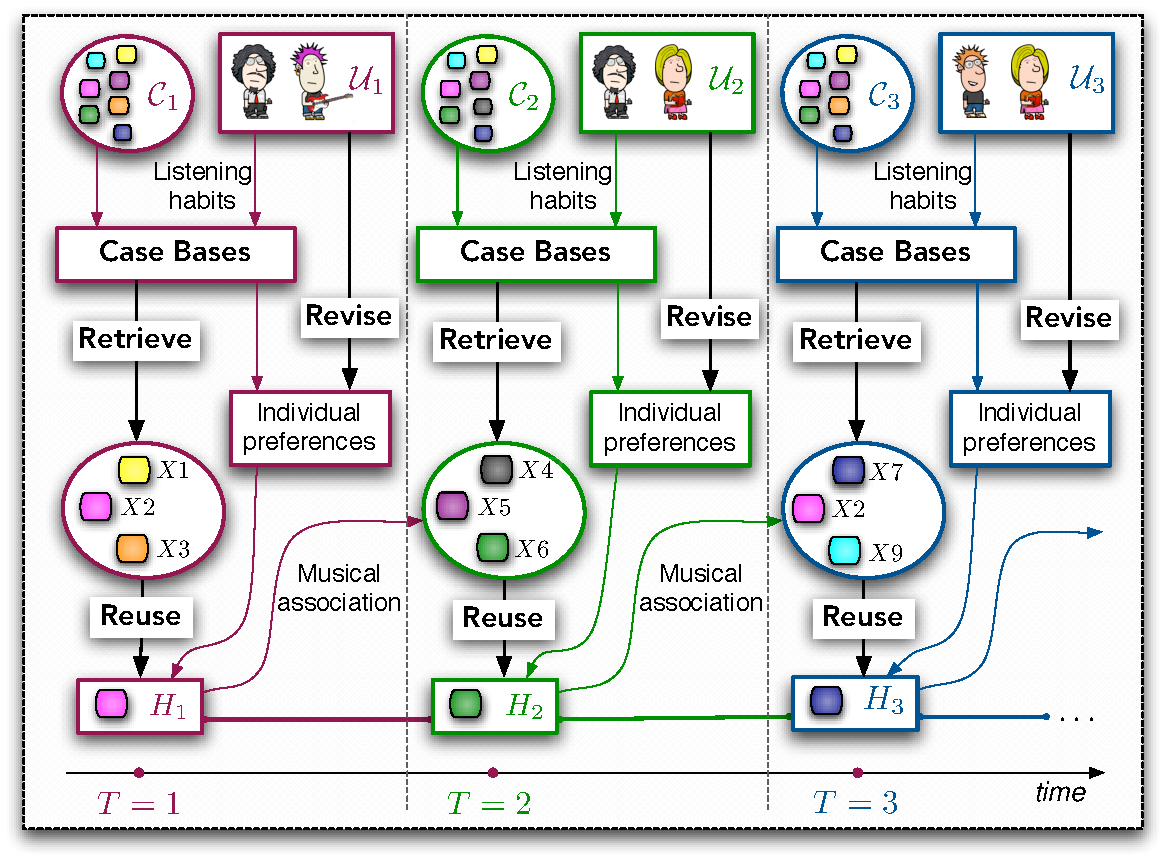
\epsfig{file=img/fig4_3, width=\textwidth}
\caption{The iterative CBR selection process.}
\label{fig:iterative_cbr}
\end{figure}





% To combine all the requirements in real time and solve the iterative social choice problem, poolcasting employs a Case-Based Reasoning (CBR) process.


% \begin{figure}[hbtp]
% \centering \setlength{\abovecaptionskip}{3pt}
% \epsfig{file=img/chap5, width=\textwidth}
% \caption{Chap 5.}
% \label{fig:chap5}
% \end{figure}



\subsection{The case bases} % (fold)
\label{sub:the_case_base_setup2}

In classical CBR, cases consist of (problem $\rightarrow$ solution) pairs;
each new problem is solved independently by retrieving similar past cases and reusing their solutions.

In poolcasting, the `problem' consists in determining which song to play at each time $T$ and cannot be solved \emph{independently} from previous and successive problems. 
In fact the objective is not to find a \emph{single} song that satisfies the audience, but to build a good \emph{sequence} of songs that fulfils variety, smoothness, customisation and fairness.

For this reason, poolcasting does not store in the case base a series of `past problems', but instead valuable knowledge to solve the sequential problem of deciding which song to play at any moment $T$.

Cases in poolcasting are defined as tuples <$X$, $a(X)$, $p(U,X,T)$>, where $X \in \mathcal{C}_T$ is any available song, $a(X)$ its performing artist, and $p(U,X,T)$ is the \textbf{individual preference} of any listener $U \in \mathcal{U}_T$ for the song $X$, that is, how much $U$ would like song $X$ to be played on the channel at time $T$.

Poolcasting is able to estimate the individual preferences of the different participants following the method presented in Chap.~\ref{cha:preferences}.
Every participant supposedly has a personal music library stored in some digital device (e.g., iPod, iTunes) and personal music libraries contain listening habits data indicating which songs a person has most played and voted.
Poolcasting extracts the listening habits data of the audience either from their music players (e.g., from Apple iTunes, see Fig.~\ref{fig:itunes_claudio}) or from the Web  (e.g., from Last.fm profiles, see Fig.~\ref{fig:lastfmprofile}) and infers the implicit preference $i(U,X)$ of each participant for each song, according to the function $i: \mathcal{U} \times \mathcal{C} \to [0,1]$ defined in \eqref{eq:implicit_preference}.
These values are then stored in the case base as individual preferences.

If a participant $V$, for instance, has `Karma Police' (Radiohead) as the top played/top rated track in the Last.fm profile page, then poolcasting stores in the case base the tuple <`Karma Police', Radiohead, 1> as a knowledge of the fact that $V$ would like that song to be played.
If a different participant $Z$ has instead a slightly negative preference for `Karma Police' (Radiohead), then poolcasting creates a second tuple <`Karma Police', Radiohead, $-0.5$> in the case base as a knowledge of the fact that $Z$ would not like that song to be played.

If two different participants have different preferences for the same song (as in the previous example), poolcasting stores both facts since they can both help decide which music to play.
To distinguish between cases related to different participants, poolcasting stores the cases of each participant in a separate case base.
In other words, poolcasting holds a \textbf{collection of case bases}, one for each participant.

%In fact, each personal music library can be seen a case base of previous experiences, namely played and rated songs. A participant sharing personal listening habits data is making available a collection of past experiences, each stored in a different case.

Each participant is treated independently and contributes with a piece of knowledge to the system.
Since participants can join and leave the channel at different moments, the collection of case bases is dynamic:
when new participants join the channel and share listening behaviour data, new case bases become available; when listeners abandon the channel, their case bases leave the collection.
The collection of case bases is determined at each moment by the songs of the current participants in the channel.

% ?? The way in which a participant shares listening habits data 

% 
% In poolcasting, past experience is related to the songs that are shared by the radio participants. 
% The shared library of each participant $U$ is considered as a Case Base, where one case corresponds to each song $X$ with its implicit preference $i(U,X)$ estimated from the analysis of the personal library as explained in Chap.N.
% 
% Every Case Base contains the list of songs in the shared library of a participant and a preference degree for each song.
% Overall, the radio has a \textbf{collection of case bases} which is dynamic because when listeners join or leave the radio and share or `unshare' their libraries, new case bases enter or leave the collection.
% 
 
% subsection the_case_base_setup2 (end)

\subsection{The retrieve process}

% When, at moment $T$, poolcasting has to decide which song to play next on the channel, it can selects one song among those available in the collection of case bases at time $T$.
% However, not \emph{all} the songs shared by the audience can be played on \emph{any} channel; for instance a channel defined as `genre = Rock' (see Fig.N) only admits `Rock' songs.
% 
% The set of songs that can actually be played on a channel at a given moment $T$ (that is, songs in shared libraries at time $T$ that match the definition of the channel) is indicated with $\mathcal{C}_T$.

The retrieve process is meant to identify at time $T$ which available songs  are \textbf{good candidates} to be played next on the channel.
The retrieve process addresses the goals of variety (\ref{p:variety}) and smoothness (\ref{p:smoothness}) with two subsequent steps: 
first each song is rated with a \emph{relevance value} $k: \mathcal{C} \times \mathbb{N}^+ \to [0,1]$ that expresses how much the song satisfies the requirements of variety and smoothness; then the $\kappa$ best rated songs are retrieved.

Every song $X \in \mathcal{C}_T$ that does not fit the channel constraints is assigned the lowest possible value $k(X,T) = 0$ to prevent that song from being played.
For instance, if a channel is defined as `Rock' then every non-Rock song gets a relevance value of 0; if a channel is defined as `Italian' then non-Italian tracks are assigned a value of $k(X,T) = 0$.

Every song recently played on the channel, or by a recently played artist, is also assigned a relevance value of 0.
This is intended to guarantee the requirement of variety.
Formally, let $H_J$ be the $J$-th song played in the channel, and let $[H_1, H_2, \ldots, H_{T-1}]$ be the list of songs played so far.
Then $k(X,T) = 0 \; \forall X \in [H_{T-\eta}, H_{T-\eta+1}, \ldots, H_{T-1}]$ (recently played songs) and $k(X,T) = 0 \; \forall X\,|\,a(X) \in [a(H_{T-\zeta}), a(H_{T-\zeta+1}), \ldots, a(H_{T-1})]$ (recently played artists).
The parameters $\eta \in \mathbb{N}^+$ and $\zeta \in \mathbb{N}^+$ determine the number of songs that have to pass before the same song or artist can be played again in the same channel.
The values of these parameters are defined according to the channel; $\zeta$ is small when the same artist is allowed to repeat (e.g., a `Frank Sinatra' channel), while a high $\eta$ characterises channels that strongly avoid repeating the same tracks (e.g. a `Dance' channel). 

Next, the retrieve process assigns a relevance value to the remaining songs according to how well they would go in a sequence after the last song played $H_{T-1}$. 
This is intended to guarantee the requirement of smoothness and is accomplished is by exploiting the co-occurrences analysis of playlists explained in Chap.~\ref{cha:smoothness}.
The idea is that the more people have played two songs together in their daily activities, the more two songs appear closely in playlists, the more they `go well' together in sequence and the more it makes sense to reproduce them one after the other in a channel to guarantee smoothness.
Formally, each remaining song $X$ in the collection of case bases is assigned a relevance value of $k(X,T) = s(H_{T-1}, X)$ that indicates how much $X$ would sound well in a sequence after the last song played $H_{T-1}$, where the function $s: \mathcal{C}^2 \to [0,1]$ was defined in \eqref{eq:final_degree}.

Having determined a relevance value $k(X,T)$ for each song $X \in \mathcal{C}_T$, the $\kappa$ songs with the highest value are identified as the best candidate songs to become $H_T$ (the next song to play).
The cases that contain these songs are retrieved and constitute the \emph{retrieved set}.

% subsection the_retrieve_process3 (end)

\subsection{The reuse process} % (fold)
\label{sub:the_reuse_process3}

The reuse process is meant to adapt the retrieved set to the preferences of the current audience. % in order to select the song that best address the requirements of customisation and fairness.
In this process, the songs in the retrieved set are \textbf{ranked} according to how much the current listeners like each song: % (\ref{p:customisation}) with an aggregation strategy defined to satisfy every listener in the long run (\ref{p:fairness}).
the top ranked song is identified as the candidate preferred by the group of listeners `as a whole'.

To know how much \emph{the group} likes each candidate song, poolcasting reuses the individual preferences $p(U,X,T)$ stored in the retrieved cases.
Every case contains knowledge about \emph{one} participant.
Poolcasting aggregates cases by candidate song to measure how much the whole group likes each candidate.


%For each candidate song $X$, poolcasting aggregates the preferences of all the current participants into a \textbf{group preference} function $g: \mathcal{C} \times \mathbb{N}^+ \to [-1,1]$ that measures how much the group `as a whole' would like to listen to a specific song $X$ at time $T$.

Several strategies exist to aggregate preferences in a group. %, which differ in the way they address the problem of fairness.
A common strategy is \emph{plurality voting}, which consists in ranking first the items preferred by the majority. 
With this approach, the preferences of the minorities never affect the determination of the best ranked item; in other words plurality voting does not endeavour to equally satisfy \emph{all} the participants.

%The main problem of plurality voting is that people with boundary preferences are completely ignored, since they do not belong to the majority.

Poolcasting uses a different strategy which combines instead the preferences of all the members of the audience, assigning more importance to those participants that were less satisfied by the last songs played.

This strategy\,---\,called satisfaction-weighted aggregation and explained in Sect.~\ref{sec:social-choice-problem}\,---\,returns for each candidate song $X$ a group preference degree $g(X,T)$ that measures how much the group as a whole would like song $X$ to be played at time $T$ on the channel.

Given this group preference function, the reuse process ranks each song $X$ in the retrieved set according to $g(X,T)$.
The best ranked song is identified as the best candidate to become $H_T$, the song that will play next on the channel.

% The `optimal' situation would be to have at least one retrieved song $Y$ that every current listener loves, that is, such as $p(U,Y,T) = 1 \forall U \in \mathcal{U}_T$. In this case, the song $Y$ would clearly be played next on the channel as this would satisfy the entire audience.
% 
% Still this situation is quite uncommon: even close friends often have different preferences for different songs and hardly one song can be found that everyone agrees upon, especially when the group is large.
% 
% In this case, the group has to accept a \textbf{compromise}: a song will be played that not everyone loves but that, hopefully, will not either be too distant from anyone's taste.
% Finding the right compromise is the most critical challenge for poolcasting: to identify the song in the retrieved set that the current audience `as a whole' most likes.
% 
% This means to combine in some way the preferences of all the listeners in order to find the retrieved song that has the highest `group preference'. 
% 
 
\subsection{The revise process} % (fold)
\label{sub:the_revise_process2}

So far, the CBR process has required no interaction from the participants.
The retrieve process has automatically picked a subset of good candidate songs that have been ranked in the reuse process according to the preferences stored in the case bases. % and the best ranked song is pre-selected to play next.
%If no additional feedback is provided, the best ranked song will be automatically uploaded to the radio server and played as soon as the previous song will have finished.

At this point, poolcasting asks the members of the audience to express feedback about the proposed ranking.
While some participants might agree with the top ranked candidate, others might prefer a different candidate song to be played.
By reviewing their preferences for the candidates, participants can alter the ranking and make a different song play next.

The revise process consists in collecting explicit feedback from the current participants about the available songs. 
\textbf{Explicit feedback} is indicated with the function $e: \mathcal{U} \times \mathcal{C} \times \mathbb{N}^+ \to [-1,1]$, where $e(U,X,T)$ denotes the last preference expressed by a participant $U$ for a song $X$ before time $T$.

The exact value of $e(U,X,T)$ depends on the type of feedback provided: $e(U,X,T) = 1$ denotes a participant $U$ who stated `unconditional love' for a song $X$; $e(U,X,T) = 0$ represents indifference; $e(U,X,T) = -1$ indicates that $U$ does not want at all $X$ to be played. 
Other values between $-1$ and $1$ mean milder negative and positive preferences. 

Explicit feedback serves to update the individual preferences $p(U,X,T)$ stored in the case bases. 
By default these preferences are inferred from personal listening habits, but if a participant explicitly states a feedback about a song, then the implicit preferences are replaced with explicit ones. 
Formally, the value of the individual preference degree $p: \mathcal{U} \times \mathcal{C} \times \mathbb{N}^+ \to [-1,1]$ is determined as follows:
\begin{equation}
\label{eq:preference_model2}
p(U,X,T) = 
\begin{cases}
e(U,X,T) & \text{if $e(U,X,T)$ is defined}\\        
i(U,X) & \text{otherwise.}
\end{cases}
\end{equation}

As listeners state their preferences for the candidate songs, the ranking calculated by the reuse process is bound to change. 
For instance, if many listeners vote positively for a given candidate song, that song might become the new top ranked candidate.
A similar outcome can occur if many participants vote negatively for the original top ranked song.

The revise process lasts for a finished period of time;
when the time is over, the best ranked song is finally confirmed as \emph{the} song $H_T$ that will play next on the channel. 
This concludes the CBR process to select the $T$-th song to play, while the process to select the $T + 1$-th song starts right after.

% subsection the_revise_process2 (end)

\section{The iterated social choice problem} % (fold)
\label{sec:social-choice-problem}


% [the key: the reuse, so decisions are not to be independent, what happens with music is that they are not independent!]

The goal of poolcasting is to generate a musical sequence customised for a given audience. 
Poolcasting determines which songs to play iterating the CBR process:
first, song $H_1$ is selected, then song $H_2$, and so on. 
%As a result, the participants get to listen to the musical sequence $[H_1, H_2, \ldots]$, automatically selected without the need for a DJ.

Each song belongs to a retrieved set of candidates that were not recently played and that go well after the last song played; this addresses the goals of variety (\ref{p:variety}) and smoothness (\ref{p:smoothness}).
Moreover each played song is the top ranked according to the combined preferences of the audience; this addresses the goal of customisation (\ref{p:customisation}).

The way in which multiple preferences are combined determines the degree in which fairness is addressed (\ref{p:fairness}).
The objective is to have every participant satisfied in the long run;
therefore if some participants are not satisfied by the music played at a given moment, poolcasting should \textbf{reward} them by playing songs they like.
In this way, everyone might listen to some of their favourite songs after a certain time.

Since the decision about which song is played is determined by the ranking of the candidate set, and since this ranking depends on the preferences of the audience, a way to reward unsatisfied participants is to aggregate preferences using a weighted average that assigns higher weights to less satisfied participants.


\subsection{Group preference degree} % (fold)
\label{sub:the_group_preference_degree}

The strategy to aggregate multiple individual preferences is called \textbf{satisfaction-weighted average}, and consists in averaging individual preferences with a weight that is inversely related to a participant's satisfaction. 

Formally, let $q(U,T)$ indicate the individual satisfaction of a participant $U$ at time $T$; the aggregated group preference is defined as:
\begin{equation}\label{eq:group_with_misery}
\sum_{U \in \mathcal{U}_T}\left( 1-q(U,T-1) \right) \cdot \cfrac{p(U,X,T)}{\#(\mathcal{U}_T)}\,.        
\end{equation}
This weighted average combines for each song $X$ the individual preferences $p(U,X,T)$ of all the members of the audience $\mathcal{U}_T$, where the weight $(1 - q(U,T-1))$ is inversely related to the satisfaction of each person.
%
The function $q(U,T)$ that measures individual satisfaction is formalised hereafter.

%A formal definition of the individual satisfaction degree $q: \mathcal{U} \times \mathbb{N}^+ \to [0,1]$ is described hereafter.

% subsection the_group_preference_degree (end)

% section the_technique (end)
\subsection{Individual satisfaction degree} % (fold)
\label{sec:calculating_individual_satisfaction}

%The first thing that is required to fairly aggregate different individual preferences is to estimate how much each listener is \emph{satisfied} with the music played so far, so that less satisfied listeners can be favoured more later on.

%The function  $q: \mathcal{U} \times \mathbb{N}^+ \to \{0,1\}$ represents the    \textbf{individual satisfaction} degree of a listener for the music played so far on a channel. The more a listener $U \in \mathcal{U}_T$ liked the songs played before time $T$, the higher the value of $q(U,T)$, and vice versa.

The individual satisfaction $q: \mathcal{U} \times \mathbb{N}^+ \to \{0,1\}$ is defined as a combination of individual preferences for the songs played so far in the channel.
In this combination, recent songs are assigned a higher importance since human satisfaction is an emotion that decays with time: people tend to forget remote experiences and be mostly affected by recent ones \cite{Masthoff06}.
The measure
\begin{equation}\label{eq:satisfaction_wrong}
  \sum_{J = 0}^{T-1} \chi^{J} p(U,H_{T-J},T-J)
\end{equation}
formalises this decay model: the individual preferences $[p(U,H_1,1)$, $p(U,H_2,2)$, $\ldots]$ of a listener $U$ for the songs played on the channel are averaged with a weight $\chi^J$ directly related to their recency, where
$\chi \in [0,1]$ is a parameter that determines the degree in which the recency of an experience influences its impact on satisfaction.
Note that when $\chi = 0$ only the last song played has an impact\footnote{When $\chi=0$, the first term of the sum contains $0^0$, which is defined as $1$ in this context.} while when $\chi = 1$ every song has equal impact.

There are three issues to consider about \eqref{eq:satisfaction_wrong}.
%
%The first issue is that the formula equals zerodoes not specify the \textbf{initial satisfaction} of the participants, that is, how satisfied a person
%
The first is that the formula combines the preferences of a participant towards \emph{all} the songs played on the channel, from $H_1$ to $H_{T-1}$.
Nevertheless, every participant is free to join and leave the channel at different moments, and only the preferences for the songs played \emph{while $U$ was listening} should determine the satisfaction of $U$.
For this reason, a \textbf{channel membership} function $m: \mathcal{U} \times \mathbb{N}^+ \to \{0,1\}$ is introduced to identify current listeners at time $T$:
\begin{equation*}
%\label{eq:channel_membership}
m(U,T) = 
\begin{cases}
1 & \text{if $U$ is a member of the channel audience at time $T$}\\        
0 & \text{otherwise}
\end{cases}
\end{equation*}
%for $T \geqslant 1$, while $m(U,0) = 1$ by convention.
and is integrated into \eqref{eq:satisfaction_wrong} to yield the formula:
\begin{equation}\label{eq:satisfaction_wrong_2}
  \sum_{J = 0}^{T-1} \chi^{J} p(U,H_{T-J},T-J) m(U,T-J)\
\end{equation}
that aggregates only the preferences of $U$ for the songs played on the channel while $U$ was listening.

%The second issue is that \eqref{eq:satisfaction_wrong_2} equals zero for every participant that has not yet listened to any song. Still, it should be accounted that people joining a channel for the first time are possibly not quite satisfied since they have not yet listened any good song. For this reason, an \textbf{initial satisfaction} degree $\iota \in [0,1]$ is  introduced that models how much each listener is satisfied at time $T = 0$. This value is integrated into \eqref{eq:satisfaction_wrong_2} and the formula rewritten as: 
%\begin{equation}\label{eq:satisfaction_wrong_3}
%  \sum_{J = 0}^{T-1} \chi^{J} p(U,H_{T-J},T-J) m(U,T-J) + \chi^{T}\iota\,.
%\end{equation}

The second issue is that \eqref{eq:satisfaction_wrong_2} yields values in the interval $[-(1-\chi)^{-1}, (1-\chi)^{-1}]$, while the desired satisfaction degree $q(U,T)$ yields values in $[0,1]$.
For this purpose, first a normalised version $h: \mathcal{U} \times \mathbb{N}^+ \to [0,1]$ of the individual preference for the played songs is defined:
\begin{equation*}
h(U,T) = \frac{1}{2} \left( p(U,H_T,T) + 1 \right) m(U,T)
\end{equation*}
where the more $U$ liked song $H_T$, the closer to 1 the value of $h(U,T)$, while $h(U,T) = 0$ if $U$ was not listening to the channel while $H_T$ was playing.
%
Next \eqref{eq:satisfaction_wrong_2} is rewritten integrating this notation, as follows:
\begin{equation*}
 \sum_{J = 0}^{T-1} \chi^{J} h(U,T-J)
\end{equation*}
and finally this measure is divided by the sum of its weights in order to yield values in $[0,1]$:
\begin{equation}\label{eq:satisfaction_wrong_4}
 \cfrac{\sum_{J = 0}^{T-1} \chi^{J} h(U,T-J)}
       {\sum_{J = 0}^{T-1} \chi^{J} m(U,T-J)}\,.
\end{equation}

The third issue is that \eqref{eq:satisfaction_wrong_4} is undefined for any participant that has not yet listened to any song, since the denominator equals zero.
To solve this problem, a default \textbf{initial satisfaction} degree $\iota \in [0,1]$ is introduced that models how satisfied a participant possibly is before listening to any song. % at time $T = 0$.
% This value is supposedly small since people joining a channel have not yet listened to any favourite song.
This value is integrated into  \eqref{eq:satisfaction_wrong_4} and the formula rewritten as:
\begin{equation*}
 \cfrac{\sum_{J = 0}^{T-1} \chi^{J} h(U,T-J) + \chi^T \iota}
       {\sum_{J = 0}^{T-1} \chi^{J} m(U,T-J) + \chi^T}\,.
\end{equation*}

This notation can be further reduced introducing the conventions that $m(U,0) = 0$ and $h(U,0) = \iota$.
Replacing in the numerator $\chi^T \iota$ with $\chi^T h(U,0)$ and, in the denominator, $\chi^T$ with $\chi^T m(U,0)$ eventually leads to define the individual satisfaction degree $q: \mathcal{U} \times \mathbb{N}^+ \to \{0,1\}$ as:
\begin{equation}
\label{eq:individual_satisfaction}
q(U,T) = \cfrac{\sum_{J = 0}^{T} \chi^{J} h(U,T-J)} {\sum_{J = 0}^{T} \chi^{J} m(U,T-J)}\,.
\end{equation}

Individual satisfaction increases whenever a song that a participant likes is played, while decreases after listening to a disliked song.
The impact of the last song played over satisfaction is not totally clear in  \eqref{eq:individual_satisfaction} but can be unfolded rewriting the function in a recursive form that defines $q(U,T)$ only from the previous satisfaction degree % at time $T>1$ 
$q(U,T-1)$ and from the preference $h(U,T)$ for the last song played:
\begin{equation}
%\label{eq:recursive_satisfaction}
   q(U,T) = q(U,T-1) + \cfrac{h(U,T) - q(U,T-1) m(U,T)} {\sum_{J=0}^{T} \chi^J m(U,T-J)} \,.
\end{equation}
This notation shows how every new song contributes with a `delta' to the satisfaction of a participant.
The impact of this delta (the second addend of the formula) is mostly determined by the decay parameter $\chi \in [0,1]$.
%
If $\chi$ is small, the impact is strong, which means that satisfaction can change rapidly over time. 
At the extreme, if $\chi = 0$, then $q(U,T) = h(U,T)$, which means the satisfaction of a participant is solely determined by the last song played.
%
On the other hand, if $\chi$ is large, then the impact is weak and satisfaction can only change slowly over time.

Figure~\ref{fig:satisfaction_decay} illustrates this behaviour with an example: 
the %red
solid line plots the preferences $h(U,T)$ of a person $U$ for 25 songs played on the channel, 
the %blue 
dotted line plots the satisfaction degree of $U$ modelled using a small decay value ($\chi = 0.2$);
the %green 
dashed line plots the same satisfaction function modelled using a large decay value ($\chi = 0.8$). 
The dotted line is sharper and responds almost immediately to the changes of $h(U,T)$, corresponding to a model of `immediate satisfaction'.
The dashed line is instead softer and more influenced by the whole history of $h(U,T)$, corresponding to a model of `long-term satisfaction'.
%
\begin{figure}[bthp]
\centering \setlength{\abovecaptionskip}{3pt}
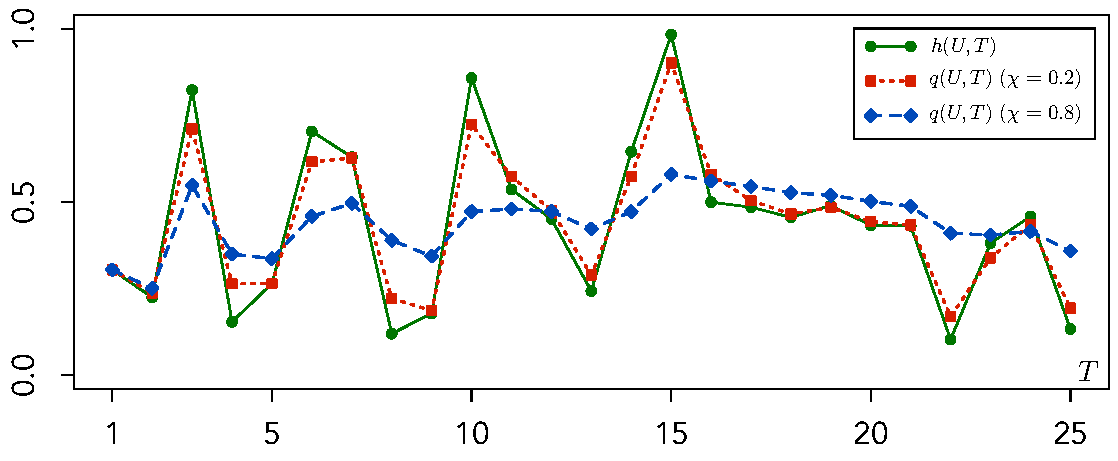
\epsfig{file=img/fig4_4, width=\textwidth}
\caption{Influence of the decay parameter $\chi$ on individual satisfaction.}
\label{fig:satisfaction_decay}
\end{figure}

% section calculating_individual_satisfaction (end)

\subsection{Satisfaction-weighted aggregation without misery} % (fold)
\label{sub:how_we_fairly_aggregate_preferences}

As defined in \eqref{eq:group_with_misery}, the individual satisfaction degree \eqref{eq:individual_satisfaction} serves to weigh the influence of different participants when deciding which song to play next on the channel.
%
This satisfaction-weighted strategy is intended to provide everyone (even participants with boundary musical tastes) with the chance to listen to some favourite songs.

One drawback of this strategy is that even songs that some participants `detest' are bound to be selected. 
In other words, the fact that a participant has the lowest possible preference $p(U,X,T) = -1$ for a given song $X$ does not prevent that song from being played if other participants with higher weights like it.
%
As a result, \emph{misery} can occur, which means that some persons are faced with items they do not wish to experience (songs they would not like to hear).

This situation can be avoided introducing a \textbf{misery threshold} $\mu \in [-1,0]$ that specifies the minimum individual preference that any member is willing to accept for a song.
If any member of the audience has a preference for a song below this threshold, then that song is not played, independently of how much the remaining audience likes that song.

Integrating this threshold into \eqref{eq:group_with_misery} brings to complete the definition of the \textbf{group preference} degree $g: \mathcal{C} \times \mathbb{N}^+ \to [-1,1]$ as:
\begin{equation*}%\label{eq:group_preference}
  g(X,T) =      
\begin{cases}
-1 & \text{if $\exists U \in \mathcal{U}_T :$}\\
& \text{$p(U,X,T) < \mu$}\\        
\rule[-1em]{0pt}{4em} 
%\displaystyle\sum_{U \in \mathcal{U}_T} \frac{q(U,T-1) + 1}{2} p(U,X,T) & 
\sum_{U \in \mathcal{U}_T}\left( 1-q(U,T-1) \right) \cdot \cfrac{p(U,X,T)}{\#(\mathcal{U}_T)} & \text{otherwise.}
\end{cases}
\end{equation*}

To conclude, the strategy of poolcasting to address customisation (\ref{p:customisation}) is to rank the retrieved set according to the group preference and to play the top ranked song.
In order to achieve fairness (\ref{p:fairness}), group preference is calculated with a weighted average that favours members that were less satisfied by the recent channel experience.
Moreover, songs with very low individual preferences are avoided to prevent misery. 

This preference aggregation strategy is iteratively used in the CBR selection process to generate a musical sequence made of songs that, over time, can satisfy the entire audience.

% subsection how_we_fairly_aggregate_preferences (end)

% section the_technique (end)



\section{Summary} % (fold)
\label{sec:contributions_c}

This chapter has described poolcasting, an automatic technique to adapt a sequence of songs to a specific audience.
Most automated music selection techniques are not influenced by the actual listeners, while poolcasting delivers a sequences of songs customised for the audience.
This is achieved by means of a CBR process, where the retrieve and reuse processes have been reinterpreted to generate a \emph{sequence} of solutions adequate for a \emph{group} of users.

The retrieve process does not look for \emph{similar} cases but searches for \emph{good candidates} for the sequence, employing the musical associations calculated in Chap.~\ref{cha:smoothness}.
The reuse process does not adapt \emph{one} retrieved case but customises the retrieved set for the audience aggregating their music profiles assessed as described in Chap.~\ref{cha:preferences}.
%In this way, I deal with the social choice problem of combining multiple individual preferences to make everyone satisfied in the long run.

%Poolcasting works in a dynamic context where members of the audience can join or leave the channel at different moments and new songs can become available over time. The preferences of the listeners are automatically inferred from listening habits and can be explicitly revised at any moment by the audience.

Multiple individual preferences are combined with a satisfaction-weighted aggregation strategy that assigns different weights to different participants based on their satisfaction degree.
The novelty of this aggregation strategy is that \emph{memory} of past elections is accounted for in order to achieve fairness in the long run.
The selection of each song depends on the previous songs selected and on their impact on listeners.
%
The outcome is that individuals might occasionally be confronted with songs they do not like to keep the rest of a group happy, but are soon rewarded with some of their favourite songs.
%The proposed strategy is particularly fit for groups willing to \emph{collaborate} and give up a bit of their individual preferences in order the make the experience satisfactory for everyone: no one will like \emph{all} the songs played, but everyone will enjoy the fact that everyone is having a good time.

The next chapter presents a real-world scenario where the poolcasting technique has been applied.

%Poolcasting avoids playing songs that any participant strongly dislikes in order to avoid misery.




% section contributions_c (end)

% subsection explicit_preferences2 (end)


%The satisfaction of each listeners for the channel at a given moment can be formalised as an \textbf{individual satisfaction} degree $q: \mathcal{U} \times \mathbb{N}^+ \to [-1,1]$, where $q(U,T)$ indicates \emph{how much} a listener $U$ is satisfied with the channel after $T$ songs have been played. Chap.N explains how poolcasting is able to estimate this degree from the analysis of the history of the individual preferences of each listener, and how satisfaction degree is used to favour at each moment less satisfied listeners in the selection of the next song to play.
% 
% 
% Processes of the CBR poolcasting technique
% 
% 
% 
% 
% \subsubsection{The Retrieve Process} % (fold)
% \label{ssub:variety}
% 
% In the retrieve process, poolcasting first excludes from $\mathcal{C}_T$ every song that has been played recently or whose artist has been played recently on the channel, then selects a set of songs which sound well after the last song played $H_{T-1}$.
% 
% In order to do this, poolcasting needs a domain knowledge about which songs sound well together after the last song played on a channel. 
% For instance, poolcasting needs to know that if `True Colors' by Cyndi Lauper is playing on a channel, then `Holiday' by Madonna is a good musical choice to play next, while `One' by Metallica is not.
% A DJ knows from experience.
% In the case of poolcasting, I will explain in Chap.N how this knowledge is automatically extracted from the analysis of playlists collected from the Web.
% Playlists are a way to organise music and poolcasting assumes that the more two songs occur closely and together in playlists, the more they sound well together. % according to a sort of `wisdom of the crowd'.
% In Chap.N we will see how analysing a large set of playlists, poolcasting is able to estimate for each pair of songs a \textbf{musical association} degree $s: \mathcal{C} \to [0,1]$ where $s(X,Y)$ measures \emph{how much} a song $Y$ sounds well after a song $X$ in a sequence.
% 
% Given this function, the songs $X \in \mathcal{C}_T$ with the highest musical association degree $s(H_{T-1}, X)$ are those that best help achieve the goal of smoothness and that are selected in the retrieve process.
% 
% % subsubsection musical_association (end)
% 
% \subsubsection{The Reuse process} % (fold)
% \label{ssub:customisation}
% 
% 
% % subsubsection fairness (end)
% 


% section what_i_want_to_do (end)


% section what_i_have_done (end)


%\section{The Case-Based Reasoning approach} % (fold)
%\label{sec:the_cbr_song_scheduler}

% The strategy of poolcasting to decide which song to play on a radio channel at a given moment is to select a song that fulfils the four requirements listed in Sect.~\ref{sec:what_i_want_to_do}: variety, smoothness, customisation and fairness.
% 
% % To fulfil variety (\ref{p:variety}), poolcasting excludes songs and artists that were recently played. For instance, if `Holiday' by Madonna is playing on a channel, poolcasting avoids playing next `Holiday' or any other song by Madonna.
% 
% 
% 
% 
%% subsection the_case_based_reasoning_approach2 (end)

